%% The first command in your LaTeX source must be the \documentclass command.
\documentclass[acmsmall]{acmart}
\usepackage{multicol}
\usepackage{wrapfig}
\usepackage{pgfplots}

%%
%% \BibTeX command to typeset BibTeX logo in the docs
\AtBeginDocument{%
  \providecommand\BibTeX{{%
    \normalfont B\kern-0.5em{\scshape i\kern-0.25em b}\kern-0.8em\TeX}}}

%% Rights management information.  This information is sent to you
%% when you complete the rights form.  These commands have SAMPLE
%% values in them; it is your responsibility as an author to replace
%% the commands and values with those provided to you when you
%% complete the rights form.
\setcopyright{rightsretained}
\copyrightyear{2021}
\acmYear{2021}
\acmDOI{}
\acmConference[Queen's University - CISC471 2021]
{Queen's University - CISC471 2021: Computational Biology}
{April 20, 2021}
{Kingston, ON, Canada}
\acmBooktitle{}
\acmPrice{}
\acmISBN{}


%%
%% Submission ID.
%% Use this when submitting an article to a sponsored event. You'll
%% receive a unique submission ID from the organizers
%% of the event, and this ID should be used as the parameter to this command.
%%\acmSubmissionID{123-A56-BU3}

%%
%% The majority of ACM publications use numbered citations and
%% references.  The command \citestyle{authoryear} switches to the
%% "author year" style.
%%
%% If you are preparing content for an event
%% sponsored by ACM SIGGRAPH, you must use the "author year" style of
%% citations and references.
%% Uncommenting
%% the next command will enable that style.
%%\citestyle{acmauthoryear}

%%
%% end of the preamble, start of the body of the document source.
\begin{document}

%%
%% The "title" command has an optional parameter,
%% allowing the author to define a "short title" to be used in page headers.
\title[Wright Fisher Algorithm with Polyploidy]{Implementation of Wright Fisher Algorithm for the Founder Effect with Polyploidy}


%%
%% The "author" command and its associated commands are used to define
%% the authors and their affiliations.
%% Of note is the shared affiliation of the first two authors, and the
%% "authornote" and "authornotemark" commands
%% used to denote shared contribution to the research.
\author{Bennet Montgomery}
\affiliation{%
  \institution{Queens University}
  \city{Kingston ON}
  \country{Canada}}
\email{bennet.montgomery@queensu.ca}

\author{Daniel Oh}
\affiliation{%
  \institution{Queens University}
  \city{Kingston ON}
  \country{Canada}}
\email{daniel.oh@queensu.ca}

\author{Evelyn Yach}
\affiliation{%
  \institution{Queens University}
  \city{Kingston ON}
  \country{Canada}}
\email{17ejy@queensu.ca}

%%
%% By default, the full list of authors will be used in the page
%% headers. Often, this list is too long, and will overlap
%% other information printed in the page headers. This command allows
%% the author to define a more concise list
%% of authors' names for this purpose.
\renewcommand{\shortauthors}{Montgomery, Oh, and Yach}

%%
%% The abstract is a short summary of the work to be presented in the
%% article.
\begin{abstract}
  Our goal is to implement and explore an algorithmic model of the Founder effect in diploid organisms using the Wright-Fisher model. We then expand on the implementation to extend its usability to organisms of an arbitrary ploidy. The base algorithm and it's extension were implemented in Python 3.8, and were designed to take input parameters modeling a hypothetical population and output the probability a recessive allele would be eliminated. Our first experiment was designed as an additional verification method, and the second as an exploration of input parameters on output. We found that the base algorithm and its extension performed well on the test cases, as well as in experiment 1. Experiment 2 found that high generations and population sizes lead to a high probability of elimination.
\end{abstract}

%%
%% The code below is generated by the tool at http://dl.acm.org/ccs.cfm.
%% Please copy and paste the code instead of the example below.
%%
\begin{CCSXML}
<ccs2012>
 <concept>
  <concept_id>10010520.10010553.10010562</concept_id>
  <concept_desc>Computer systems organization~Embedded systems</concept_desc>
  <concept_significance>500</concept_significance>
 </concept>
 <concept>
  <concept_id>10010520.10010575.10010755</concept_id>
  <concept_desc>Computer systems organization~Redundancy</concept_desc>
  <concept_significance>300</concept_significance>
 </concept>
 <concept>
  <concept_id>10010520.10010553.10010554</concept_id>
  <concept_desc>Computer systems organization~Robotics</concept_desc>
  <concept_significance>100</concept_significance>
 </concept>
 <concept>
  <concept_id>10003033.10003083.10003095</concept_id>
  <concept_desc>Networks~Network reliability</concept_desc>
  <concept_significance>100</concept_significance>
 </concept>
</ccs2012>
\end{CCSXML}

\ccsdesc[500]{Applied computing~Life and medical sciences}
\ccsdesc[300]{Applied computing~Genomics}
\ccsdesc{Mathematics of computing~Statistics}
%%\ccsdesc[100]{Networks~Network reliability}

%%
%% Keywords. The author(s) should pick words that accurately describe
%% the work being presented. Separate the keywords with commas.
\keywords{wright-fisher, allele inheritance, ploidy}

%%
%% This command processes the author and affiliation and title
%% information and builds the first part of the formatted document.
\maketitle

%% MULTI COLUMNNNNNNNN
\begin{multicols}{2}

\section{Introduction}
The Founder effect refers to the principle in genetic analysis that the proportion of a mutation can be radically altered in a small population, usually one that has been separated from a larger more diverse population. An example of this would be the complete elimination of a specific allele in a Founder population after just a few generations. Modelling the Founder effect could be a valuable tool in population genetics, allowing researchers to determine the likelihood that a specific allele is eliminated or otherwise radically changed in proportion to the parent population. The Wright-Fisher model can be used for this purpose. \par
The Wright-Fisher model assumes a population will have discrete non-overlapping generations and that each generation all individuals are replaced by the members of the next generation. The model also assumes that parents are chosen completely at random from the previous generation for each individual. Given all of these assumptions, the probability $P_{ij}$ of a given allele with incidence $i$ in the previous generation having incidence $j$ in this generation of a diploid species of population $N$ is defined by the formula: $P_{ij} = {2N\choose j} (i/2N)^j (1-i/2N)^{2N-j}$. \par
Our algorithm uses the Wright-Fisher model to determine the probability of an allele or set of alleles being eliminated at or before a generation as required by the Rosalind problem FOUN\footnote{http://rosalind.info/problems/foun/}. Each generation, a distribution of probabilities are generated, one for each potential value of $j$. These probabilities are based on the distribution for the previous generation. The first such distribution is calculated using the known initial values of allele incidence given as input to the algorithm. \par
This algorithm is preferable to the alternative approach of simulating allele inheritance. In that approach, each generation new organisms are generated with randomly selected parents from the previous generation. The simulation is run hundreds or thousands of times and the average generation in which each allele is eliminated is used to calculate the probability of elimination. This is an inferior method due to its much higher time complexity relative to the Wright-Fisher based algorithm. The Wright-Fisher based algorithm has a time complexity $O(m \times 2N)$ for each allele where $m$ is the generation count and $N$ is the population while the alternative approach has a time complexity of $O(i \times m \times 2N)$ where $i$ is the number of simulations, $m$ is the generation count, and $N$ is the population for each allele. \par
The Wright-Fisher algorithm can also be extended to work for an arbitrary n-ploidy organism. The binomial equation used to find the the probability distribution for diploids can be retooled to work for other n-ploidy organisms, extending the algorithm use case significantly.

\section{Related Work}
%% the Founder effect discovery  have been a disaster for the human race
The Founder effect was first proposed in 1942 by Ernest Mayr, who described it as a the phenomenon of new populations being distinctively different from others as a result of low genetic variance\cite{mayr1942}. Clegg et al studied the natural colonization events by the silvereye species-complex (Zosterops lateralis) and concluded that "four to five successive Founder events are required before indices of diversity and divergence approach that seen in evolutionarily old forms"\cite{clegg2002}. Peter and Slatkin studied the effective Founder effect that was taking place in spatially expanding populations\cite{peter2015}. They developed a model to reflect different amounts of genetic drift experienced by different sub-populations and found that the average strength of the Founder effect in the Americas was 3 times that of Europe. \par

%% and its consequences (tristan de cunha etc)
Understanding and modeling the Founder effect is important for medical science and genetics, and multiple historical examples have been recorded in human populations. One of the most well known cases of this includes the Amish population in Pennsylvania, who experience various genetic diseases such as Ellis-van Creveld (EvC) syndrome as stated by McKusick\cite{mckusik2000}. An example which outlines impact of the Founder effect in terms of genetic diseases were observed in the Tristan De Cunha population by Thompson who determined that the local population has a much higher frequency of retinitis pigmentosa when compared to the world population\cite{thompson1978}. The Hasidic population of Orthodox Jewish people are also a canonical example of the Founder effect, their community's intensely insular nature leading to high expression of otherwise rare allele linked disorders\cite{medintz1998}. A community in the southwest of the Netherlands has been recorded to have a significantly smaller number of or even 0 incidence of 592 surveyed genetic markers in a test done in 2005\cite{pardo2005}. \par

%% have been a disaster for the human race (new and ongoing concerns)
In the present day, studying the Founder effect has several important applications. In the field of agriculture, it has been observed that many crop species originated from a very small sample of the plant's wild population. This has far reaching implications on the stability and viability of several staple crop species\cite{ladizinsky1985}. Research into the Founder effect in polyploids has been done extensively in botany as many plants are triploids or tetraploids\cite{thompson1992}. An algorithmic extension of Wright-Fisher to polyploidy may be of great interest to this field. Finally, the impact of the Founder effect has important effects on epidemiology of SARS-CoV-2. Research has been done in studying the genetic imprint left by the Founder effect in an outbreak region to determine where that outbreak spread from\cite{ruan2020}. 

\section{Approach}
\subsection{Main Algorithm}
The Wright-Fisher algorithm was implemented in Python 3.8. The algorithm takes some population number $N$, some number of generations $m$, and an array of initial allele incidences $A$. Each allele in $A$ is considered independent of all other alleles in $A$. \par
The algorithm considers each allele in $A$ separately, passing the incidence for each row and the input parameters to a function $WFMD()$, a solution to the Rosalind WFMD node\footnote{http://rosalind.info/problems/wfmd/} that we need. For the first calculated generation, a probability distribution representing all potential incidences is calculated given the starting incidence of the allele as the previous incidence in the Wright-Fisher formula. This distribution is set to $prev\_distribution$ and the value of the probability of the allele having 0 incidence in the first generation is stored. \par
For the remainder of the generations, the distribution is calculated using the $prev\_distribution$ in combination with the Wright-Fisher formula. For each $j$ in the new distribution, the probability is equal to the probability of that $j$ being selected given $i$ was the previous incidence times the probability that $i$ was the previous incidence taken from $prev\_distribution$. After the new distribution is built, this distribution is set to $prev\_distribution$ and the value of the probability of the allele having 0 incidence in this generation is stored. Finally, the list of probabilities of 0 incidence by generation are returned. Once all allele distributions are calculated, the algorithm constructs an array with the data returned in the format expected by the Rosalind $FOUN$ problem. \par
Verification of the main algorithm is done through a unit test suite implemented in the unittest package in Python 3. Six unit tests were used to verify the main algorithm, three of which were dedicated to verifying the utility function $WFMD()$. These tests covered the default data from Rosalind for both the $FOUN$ problem and the $WFMD$ problem, cases for which had to have their expected value calculated by hand, and an edge case in which the allele being tracked started with incidence 0. 
Further verification was accomplished through Experiment 1, which compared the output of the algorithm to a simulation of allele inheritance run 75000 times. This was done to check the results of our algorithm against a solution that certainly works for this problem but is much less efficient. 

\subsection{Extension}
An extension to algorithm was made to allow for arbitrary ploidy in an organism's genome. This was done with a key observation regarding the Wright-Fisher model function $P_{ij} = {2N\choose j} (i/2N)^j (1-i/2N)^{2N-j}$, namely that this function is based on the binomial coefficient. Because of this, we can alter the model function for any ploidy by changing the internal variables in this function to $P_{ij} = {pN\choose j} (i/pN)^j (1-i/pN)^{pN-j}$ where $p$ is the ploidy of the organism. This should give us the probability of an allele appearing with incidence $j$ given previous incidence $i$ for any ploidy $p$. \par
The algorithm for Wright-Fisher using this new generalized formula could no longer rely on $WFMD()$, as $WFMD()$ specifically assumes that the organism is diploid. As a result, the algorithm had to be completely rewritten with all incidences of the formula and all places where diploidy was assumed redone to fit our revised Wright-Fisher formula. 
The correctness of the extension implementation was verified with unit tests implemented in the Python 3 unittest framework, with a total of two such tests specifically dedicated to the extension. The first of these tests checked that the extension worked on cases covered by the main algorithm (diploid organisms) and the second tested the extension on a test case for which the expected results needed to be hand calculated. \par
As with the main algorithm, the extension was further verified in Experiment 1 by comparing it to an allele inheritance simulation for a polyploid species. This simulation was run 75000 times and its output checked against the output of the main algorithm extension. 

\subsection{Experiment 1}
The main goal of our first experiment will be to confirm the correctness of our Wright Fisher Founder effect algorithm via the use of an allele simulation program. This allele simulation will take the same input as our Wright Fisher Founder effect algorithm and simulate the alleles in a neutral environment. As with the assumptions made for the Wright-Fisher Founder effect algorithm, this simulation will also assume that organism population will stay constant throughout all generations. The important aspect of this assumption is that this means the total number of alleles will also stay constant throughout generations, meaning that we can more efficiently simulate alleles instead of entire individuals. As a by-product of this study, we hope that our implementation of an allele simulator can be useful in the future when researching allele distribution and the Founder effect.\par
When generating each new generation, each allele is randomly assigned a 0 or a 1. A 0 means the allele is a dominant allele, while a 1 means it is recessive. This randomness is influenced by the last generation�s recessive to total allele ratio. For example, if 40\% of the alleles in the last generation were recessive, then each allele in the new generation will have a 40\% chance to be recessive, and a 60\% chance to be dominant. We chose to implement this as a random function instead of simply setting 40\% of the new generation to be recessive because then we would not be able to measure the frequency of the possibility of all recessive alleles disappearing in the early generations. Also, if the recessive allele count was greater than 50\% of the total alleles, then it would be impossible for the recessive allele frequency to reach 0. Since the chance of all recessive alleles disappearing is the main variable we measure, it is critical that it represented by a random function.\par
Once all the generations have been simulated, each generation and their alleles are recorded, and the simulation restarts. The encompassing program runs many identical iterations of the simulation as to receive a reliable average in the end. The data returned from the program is then processed into an array identical to that of the array returned by the Wright Fisher Founder effect algorithm, a 2D $ixj$ list of log10 of probabilities that $j$ allele is eliminated in or before generation $i$.\par
When the implementation of the allele simulation is complete, the simulation will be run side by side with the Wright Fisher Founder effect algorithm with the exact same parameters. For a recap, the parameters include population size $N$, number of generations $m$, recessive alleles per gene $A$, and ploidy $p$. There will be 4 tests, each changing a single variable 3 times. The output will be directly compared to each other in a table where we can determine if the Wright Fisher Founder effect algorithm is accurate.

\subsection{Experiment 2}
The second experiment we conducted explored the variance of the base algorithms input parameters. The parameters that underwent variance was the number of individuals in a population ($N$), the number of generations ($m$), and an array containing the number of recessive alleles for each factor in the population ($A$). To test the effect of the population size parameter, the algorithm was run on a constant m set to 5, and each instance in $A$ ranging from 0-5, was compared at $N$ values ranging from 5 to 160. This allowed for the examination of the effect of a growing population on the probability of a recessive allele persisting within the population. \par
The next test of parameter effect consists of increasing the number of generations used, and examining its effect on the recessive allele frequency of the population. This was achieved by running the base algorithm once on an $m$ of 10, and each instance of $A$ ranging from 0-9, with a fixed $N$ of 10. This allowed for the cross evaluation of the probability that an allele would be lost across a large number of generations. As well as the effect of an increased number of recessive alleles across a single generation. Both of these within the context of a fixed number of individuals across generations.

\section{Results and Discussion}
\subsection{Main Algorithm}
Following implementation, the time taken to run the main algorithm on the Rosalind default data for the $FOUN$ problem was $7.371 \times 10^{-2}$ seconds on a machine with an AMD Ryzen 5 3600 6-core processor and 16 gigabytes of RAM. The algorithm passed all 6 unit tests. The main algorithm was also successfully verified by output comparison in experiment 1. As the algorithm passed all unit tests and was checked against experimental data, we are confident that it works in all diploid cases.

\subsection{Extension}
Following implementation, the time taken to run the algorithm with extension on the Rosalind default data for the $FOUN$ problem was $4.637 \times 10^{-2}$ seconds on a machine with an AMD Ryzen 5 3600 6-core processor and 16 gigabytes of RAM. The Extension passed both unit tests, including the one testing it for coverage of problems covered by the original algorithm. The extension was also successfully verified by output comparison in experiment 1. \par
The extension was most likely faster than the main algorithm due to the necessity of rewriting the entire algorithm, as $WFMD()$ could not be used as a utility function. As a result, the extension did not have to wait for a function call to execute nor did it have to dedicate extra instructions to converting output data from $WFMD()$ to the data format required by the $FOUN$ problem. \par
The fact that the extension passed the unit test for diploid organisms implies that it also works on all cases covered by the original algorithm. The only change between the two algorithms is the rework from diploid only to arbitrary ploidy for the extension. In fact, not only does our extension extend coverage of the algorithm, it does it faster than the original $WFMD()$ reliant implementation.

\subsection{Experiment 1}
\begin{table*}
    \caption{Comparison of the output when changing $N$ and having $m = 3$, $A = [0, 1, 2]$, and $p = 2$. The simulator runs for 75000 iterations. The output was edited to 4 decimal places.}
    \label{tab:changeN}
    \begin{tabular}{ccl}
        \toprule
            $N$&Wright Fisher Founder effect algorithm output&Allele simulator output\\
        \midrule
            4 & \begin{tabular}[c]{@{}l@{}}{[}{[} 0.     -0.4639 -0.9995{]}\\  {[} 0.       -0.3014 -0.6417{]}\\  {[} 0.       -0.2291 -0.4858{]}{]}\end{tabular} & \begin{tabular}[c]{@{}l@{}}{[}{[} 0.     -0.4639 -1.0013{]}\\  {[} 0.       -0.3024 -0.6409{]}\\  {[} 0.       -0.2299 -0.4839{]}{]}\end{tabular} \\
        \midrule
            5 & \begin{tabular}[c]{@{}l@{}}{[}{[} 0.     -0.4576 -0.9691{]}\\  {[} 0.       -0.2956 -0.6204{]}\\  {[} 0.       -0.2235 -0.4677{]}{]}\end{tabular} & \begin{tabular}[c]{@{}l@{}}{[}{[} 0.     -0.4569 -0.9672{]}\\  {[} 0.       -0.2946 -0.6187{]}\\  {[} 0.       -0.2236 -0.4644{]}{]}\end{tabular} \\
        \midrule
            6 & \begin{tabular}[c]{@{}l@{}}{[}{[} 0.     -0.4535 -0.9502{]}\\  {[} 0.       -0.2919 -0.6071{]}\\  {[} 0.       -0.2199 -0.4564{]}{]}\end{tabular} & \begin{tabular}[c]{@{}l@{}}{[}{[} 0.     -0.4517 -0.9527{]}\\  {[} 0.       -0.2914 -0.6067{]}\\  {[} 0.       -0.2186 -0.4558{]}{]}\end{tabular}\\
        \bottomrule
    \end{tabular}
\end{table*}

\begin{table*}
    \caption{Comparison of the output when changing $p$ and having $N = 4$, $m = 3$, $A = [0, 1, 2]$. The simulator runs for 75000 iterations. The output was edited to 4 decimal places.}
    \label{tab:changeP}
    \begin{tabular}{ccl}
        \toprule
            $P$&Wright Fisher Founder effect algorithm output&Allele simulator output\\
        \midrule
            2 & \begin{tabular}[c]{@{}l@{}}{[}{[} 0.     -0.4639 -0.9995{]}\\  {[} 0.       -0.3014 -0.6417{]}\\  {[} 0.       -0.2291 -0.4858{]}{]}\end{tabular} & \begin{tabular}[c]{@{}l@{}}{[}{[} 0.     -0.4651 -0.9988{]}\\  {[} 0.       -0.3022 -0.6414{]}\\  {[} 0.       -0.2303 -0.4868{]}{]}\end{tabular} \\
        \midrule
            3 & \begin{tabular}[c]{@{}l@{}}{[}{[} 0.     -0.4535 -0.9502{]}\\  {[} 0.       -0.2919 -0.6071{]}\\  {[} 0.       -0.2199 -0.4564{]}{]}\end{tabular} & \begin{tabular}[c]{@{}l@{}}{[}{[} 0.     -0.4556 -0.9415{]}\\  {[} 0.       -0.2926 -0.6031{]}\\  {[} 0.       -0.2209 -0.4547{]}{]}\end{tabular} \\
        \midrule
            4 & \begin{tabular}[c]{@{}l@{}}{[}{[} 0.     -0.4485 -0.9279{]}\\  {[} 0.       -0.2873 -0.5914{]}\\  {[} 0.       -0.2156 -0.4429{]}{]}\end{tabular} & \begin{tabular}[c]{@{}l@{}}{[}{[} 0.     -0.4515 -0.9283{]}\\  {[} 0.       -0.2877 -0.5901{]}\\  {[} 0.       -0.2162 -0.4436{]}{]}\end{tabular}\\
        \bottomrule
    \end{tabular}
\end{table*}

\begin{table*}
    \caption{Comparison of the output when changing $A$ and having $N = 4$, $m = 3$, and $p = 2$. The simulator runs for 75000 iterations. The output was edited to 4 decimal places.}
    \label{tab:changeA}
    \begin{tabular}{ccl}
        \toprule
            $A$&Wright Fisher Founder effect algorithm output&Allele simulator output\\
        \midrule
            {[}0, 1,  2{]}      & \begin{tabular}[c]{@{}l@{}}{[}{[} 0.     -0.4639 -0.9995{]}\\  {[} 0.       -0.3014 -0.6417{]}\\  {[} 0.       -0.2291 -0.4858{]}{]}\end{tabular}                                                 & \begin{tabular}[c]{@{}l@{}}{[}{[} 0.     -0.4710 -0.9940{]}\\  {[} 0.       -0.3061 -0.6389{]}\\  {[} 0.       -0.2317 -0.4841{]}{]}\end{tabular}\\
        \midrule
            {[}0, 1, 2, 3{]}    & \begin{tabular}[c]{@{}l@{}}{[}{[} 0.     -0.4639 -0.9995 -1.6330{]}\\  {[} 0.       -0.3014 -0.6417 -1.0334{]}\\  {[} 0.       -0.2291 -0.4858 -0.7789{]}{]}\end{tabular}                         & \begin{tabular}[c]{@{}l@{}}{[}{[} 0.     -0.4610 -1.0009 -1.6428{]}\\  {[} 0.       -0.3015 -0.6443 -1.0350{]}\\  {[} 0.       -0.2284 -0.4884 -0.7835{]}{]}\end{tabular}\\
        \midrule
            {[}0, 1, 2, 3, 4{]} & \begin{tabular}[c]{@{}l@{}}{[}{[} 0.     -0.4639 -0.9995 -1.6330 -2.4082{]}\\  {[} 0.       -0.3014 -0.6417 -1.0334 -1.4970{]}\\  {[} 0.       -0.2291 -0.4858 -0.7789 -1.1222{]}{]}\end{tabular} & \begin{tabular}[c]{@{}l@{}}{[}{[} 0.     -0.4664 -0.9962 -1.6273 -2.3979{]}\\  {[} 0.       -0.3013 -0.6410 -1.0259 -1.5029{]}\\  {[} 0.       -0.2285 -0.4868 -0.7713 -1.1199{]}{]}\end{tabular}\\
        \bottomrule
    \end{tabular}
\end{table*}

\begin{table*}
    \caption{Comparison of the output when changing $N$ and having $m = 3$, $A = [0, 1, 2]$, and $p = 2$. The simulator runs for 75000 iterations. The output was edited to 4 decimal places.}
    \label{tab:changeM}
    \begin{tabular}{ccl}
        \toprule
            $m$&Wright Fisher Founder effect algorithm output&Allele simulator output\\
        \midrule
            3 & \begin{tabular}[c]{@{}l@{}}{[}{[} 0.     -0.4639 -0.9995{]}\\  {[} 0.       -0.3014 -0.6417{]}\\  {[} 0.       -0.2291 -0.4858{]}{]}\end{tabular}                                                                       & \begin{tabular}[c]{@{}l@{}}{[}{[} 0.     -0.4645 -1.0024{]}\\  {[} 0.       -0.3010 -0.6464{]}\\  {[} 0.       -0.2292 -0.4869{]}{]}\end{tabular}\\
        \midrule
            4 & \begin{tabular}[c]{@{}l@{}}{[}{[} 0.     -0.4639 -0.9995{]}\\  {[} 0.       -0.3014 -0.6417{]}\\  {[} 0.       -0.2291 -0.4858{]}\\  {[} 0.       -0.1873 -0.3966{]}{]}\end{tabular}                                    & \begin{tabular}[c]{@{}l@{}}{[}{[} 0.     -0.4636 -1.0044{]}\\  {[} 0.       -0.3008 -0.6438{]}\\  {[} 0.       -0.2285 -0.4889{]}\\  {[} 0.       -0.1867 -0.3989{]}{]}\end{tabular}\\
        \midrule
            5 & \begin{tabular}[c]{@{}l@{}}{[}{[} 0.     -0.4639 -0.9995{]}\\  {[} 0.       -0.3014 -0.6417{]}\\  {[} 0.       -0.2291 -0.4858{]}\\  {[} 0.       -0.1873 -0.3966{]}\\  {[} 0.       -0.1600 -0.3385{]}{]}\end{tabular} & \begin{tabular}[c]{@{}l@{}}{[}{[} 0.     -0.4673 -0.9936{]}\\  {[} 0.       -0.3042 -0.6422{]}\\  {[} 0.       -0.2313 -0.4863{]}\\  {[} 0.       -0.1897 -0.3970{]}\\  {[} 0.       -0.1621 -0.3389{]}{]}\end{tabular}\\
        \bottomrule
    \end{tabular}
\end{table*}
Comparing the results of both programs next to each other, we can see a striking similarity in their outputs. For each value in the return arrays of the Wright Fisher Founder effect algorithm, there is a near identical value in the Allele simulator return array, with a small margin of error. However, this error does not exceed � 0.01 in any instance. With this, we can confidently say that we have supplied sufficient evidence to imply that our implementation of the Wright Fisher Founder effect algorithm is correct.\par
Comparing the Wright Fisher Founder effect algorithm to our Allele simulator gives us the opportunity to discuss the strengths and weaknesses of the program. A general comparison can be made stating that the Allele simulator is more akin to a �brute force� version of the Wright Fisher Founder effect algorithm. This already gives the obvious disadvantage in efficiency and speed to the Allele simulator. Our implementation of the Allele simulator is an $O(n^4)$ algorithm, where the main factors for run-time are the number of iterations to run, number of generations, number of genes, and finally the total number of alleles. Despite the time complexity of the Allele simulator being close to the Wright Fisher Founder effect algorithm, the Allele simulator performs worse on average. The Allele simulator requires a very high number of iterations no matter how small the input values are, as it relies on high amounts of data to arrive at a reasonable final mean. For our experiment, the number of iterations had been set to 75000. Despite this, there still existed a small yet noticeable error. As the Wright Fisher Founder effect algorithm has no error values, any output with noticeable error should be scrutinized. With this, it is evident that the Wright Fisher Founder effect algorithm has a significant advantage over a brute force method. Anyone looking to implement either or these algorithms or similar should opt to implement the Wright Fisher Founder effect algorithm.

\subsection{Experiment 2}
The results of varying the number of generations ($m$) is illustrated in Figure \ref{fig:vary_m}. The values on the x-axis represent the probability a recessive allele will be lost. The values returned from the base algorithm are $log10$, but here on the graph the absolute value has been taken of each of them for readability. The y-axis represents the number of recessive alleles in a generation. Each coloured line then corresponds to a generation, a total of 10 were recorded. This was due to the diminishing differences in probabilities from higher generation counts.\par

\begin{figure*}[!ht]
    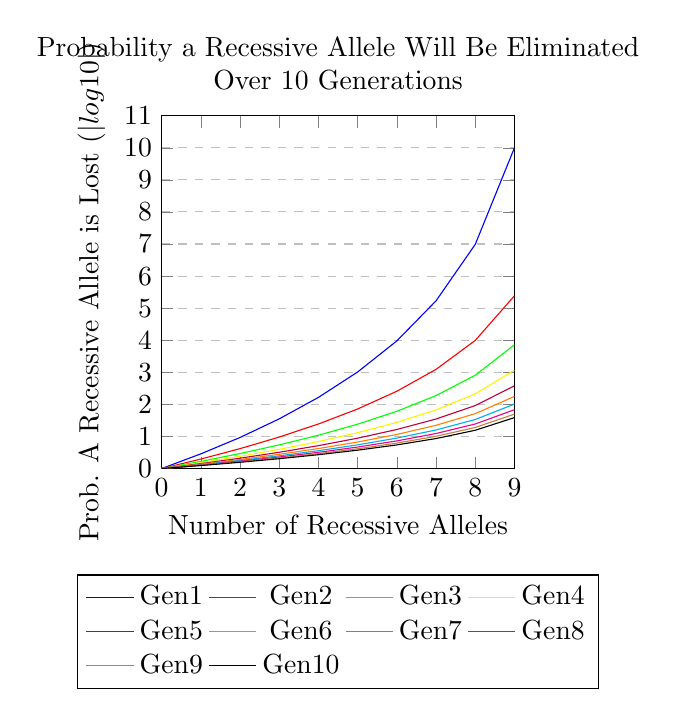
\begin{tikzpicture}
        \begin{axis}[
            width=0.5\textwidth,
            height=0.5\textwidth,
            title style={align=center}, title={Probability a Recessive Allele Will Be Eliminated \\Over 10 Generations},
            xlabel={Number of Recessive Alleles},
            ylabel style={align=center}, ylabel={Prob. A Recessive Allele is Lost ($|log10|$)},
            xmin=0, xmax=9,
            ymin=0, ymax=11,
            xtick={0,1,2,3,4,5,6,7,8,9},
            ytick={0,1,2,3,4,5,6,7,8,9,10,11},
            ymajorgrids=true,
            grid style=dashed,
            legend style={
                at={(0.5,-0.3)},
        	    anchor=north,
        	    legend columns=4
        	},
        ]
        
        \addplot[color=blue]
            coordinates{
             (0,0)(1,0.45757491)(2,0.96910013)(3,1.5490196)(4,2.2184875)(5,3.01029996)(6,3.97940009)(7,5.22878745)(8,6.98970004)(9,9.99999996)
            };
        \addplot[color=red]
            coordinates{
             (0,0)(1,0.29563211)(2,0.62043397)(3,0.98138417)(4,1.38844008)(5,1.85657829)(6,2.41000051)(7,3.09210204)(8,3.99478059)(9,5.38670994)
            };
        \addplot[color=green]
            coordinates{
             (0,0)(1,0.22351583)(2,0.46769705)(3,0.73730864)(4,1.03909605)(5,1.38311268)(6,1.78542959)(7,2.27448199)(8,2.90944762)(9,3.85891762)
            };
        \addplot[color=yellow]
            coordinates{
             (0,0)(1,0.18189307)(2,0.38008162)(3,0.59826276)(4,0.84165337)(5,1.11799988)(6,1.4396319)(7,1.82824991)(8,2.32870762)(9,3.06746307)
            };
        \addplot[color=purple]
            coordinates{
             (0,0)(1,0.15461141)(2,0.32284438)(3,0.50776711)(4,0.71370367)(5,0.94706641)(6,1.21804684)(7,1.54455467)(8,1.96355482)(9,2.57939167)
            };
        \addplot[color=orange]
            coordinates{
             (0,0)(1,0.13529481)(2,0.28240517)(3,0.44398603)(4,0.62377886)(5,0.82733233)(6,1.0634687)(7,1.34770938)(8,1.71220127)(9,2.24885243)
            };
        \addplot[color=cyan]
            coordinates{
             (0,0)(1,0.12088543)(2,0.25228658)(3,0.39656786)(4,0.55706365)(5,0.73872457)(6,0.94943732)(7,1.2031284)(8,1.52886758)(9,2.01137344)
            };
        \addplot[color=magenta]
            coordinates{
             (0,0)(1,0.10972389)(2,0.22898601)(3,0.35993713)(4,0.50561469)(5,0.67053812)(6,0.86193187)(7,1.09262741)(8,1.38969221)(9,1.83361322)
            };
        \addplot[color=brown]
            coordinates{
             (0,0)(1,0.10082848)(2,0.21043648)(3,0.33081311)(4,0.46477345)(5,0.61651901)(6,0.79279727)(7,1.00567899)(8,1.28091743)(9,1.69646887)
            };
        \addplot[color=black]
            coordinates{
             (0,0)(1,0.09357995)(2,0.1953368)(3,0.30713517)(4,0.43162123)(5,0.57275962)(6,0.73695195)(7,0.93573814)(8,1.19400428)(9,1.58816955)
            };
        \legend{Gen1, Gen2, Gen3, Gen4, Gen5, Gen6, Gen7, Gen8, Gen9, Gen10}
            
        \end{axis}
    \end{tikzpicture}
    
    \caption{Line graph illustrating the probability of an allele persisting, each coloured line corresponds to a generation in the population.}
    \label{fig:vary_m}
\end{figure*}

The results of varying the number of individuals ($N$) is illustrated in Figure \ref{fig:vary_N}. The values on the x-axis represent the probability a recessive allele will be lost. The values returned from the base algorithm are $log10$, but graphed is the absolute value that has been taken of each of them for readability purposes. The y-axis represents the number of recessive alleles in a generation. Each coloured line then corresponds to a population size.\par

\begin{figure*}[!ht]
    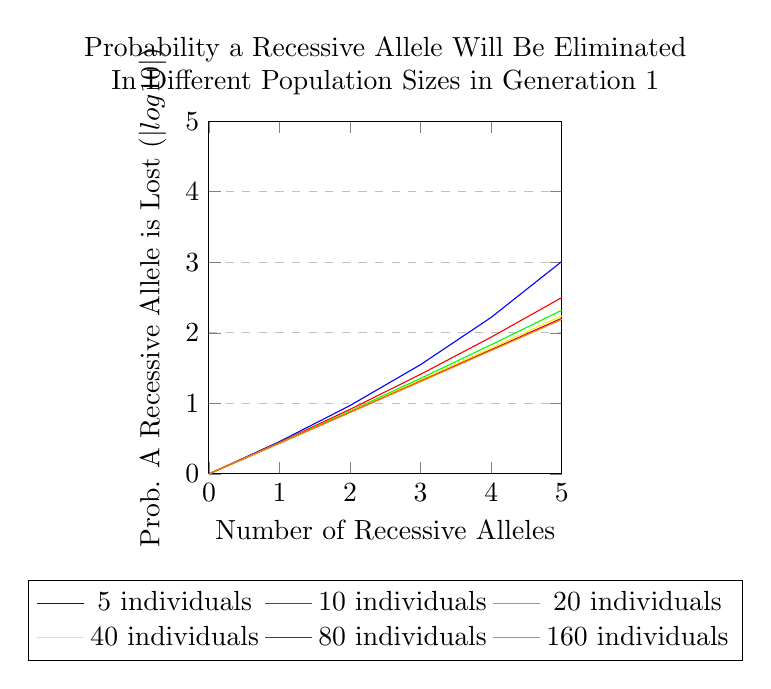
\begin{tikzpicture}
        \begin{axis}[
            width=0.5\textwidth,
            height=0.5\textwidth,
            title style={align=center}, title={Probability a Recessive Allele Will Be Eliminated \\In Different Population Sizes in Generation 1},
            xlabel={Number of Recessive Alleles},
            ylabel style={align=center}, ylabel={Prob. A Recessive Allele is Lost ($|log10|$)},
            xmin=0, xmax=5,
            ymin=0, ymax=5,
            xtick={0,1,2,3,4,5},
            ytick={0,1,2,3,4,5},
            ymajorgrids=true,
            grid style=dashed,
            legend style={
                at={(0.5,-0.3)},
        	    anchor=north,
        	    legend columns=3
        	},
        ]
        
        \addplot[color=blue]
            coordinates{
             (0,0)(1,0.45757491)(2,0.96910013)(3,1.5490196)(4,2.2184875)(5,3.01029996)
            };
        \addplot[color=red]
            coordinates{
             (0,0)(1,0.44552789)(2,0.91514981)(3,1.41162149)(4,1.93820026)(5,2.49877473)
            };
        \addplot[color=green]
            coordinates{
             (0,0)(1,0.43981537)(2,0.89105579)(3,1.35433069)(4,1.83029962)(5,2.31967788)
            };
        \addplot[color=yellow]
            coordinates{
             (0,0)(1,0.43703166)(2,0.87963074)(3,1.32794095)(4,1.78211158)(5,2.24229789)
            };
        \addplot[color=purple]
            coordinates{
             (0,0)(1,0.43565733)(2,0.87406331)(3,1.31525284)(4,1.75926149)(5,2.20612552)
            };
        \addplot[color=orange]
            coordinates{
             (0,0)(1,0.43497448)(2,0.87131467)(3,1.30902915)(4,1.74812662)(5,2.18861585)
            };
        \legend{5 individuals, 10 individuals, 20 individuals, 40 individuals, 80 individuals, 160 individuals}
            
        \end{axis}
    \end{tikzpicture}
    
    \caption{Line graph illustrating the probability of an allele persisting, each coloured line corresponds to the size of the population.}
    \label{fig:vary_N}
\end{figure*}

Examining the results above, we can see a number of trends emerge in Figure \ref{fig:vary_m}. Firstly with an increasing number of recessive alleles, the probability that a recessive allele is lost increases. This is supported by a similar trend in Figure \ref{fig:vary_N}. This can be attributed to an increased amount of competition among the recessive alleles in the population.\par
Further examination of Figure \ref{fig:vary_m}, leads to the conclusion that there is a distinct pattern in the generation number and the probability of a recessive allele being lost. A recessive allele in an earlier generation has a higher probability of being eliminated then one in a later generation. Considering the Founder effect, this particular trend makes sense, as genetic diversity tends to dwindle with an increased number of generations. This notion is further supported by "single Founder events do not affect levels of heterozygosity or allelic diversity ... four to five successive Founder events are required"\cite{clegg2002}.\par

Moving onto Figure \ref{fig:vary_N}, we see similar trends as Figure \ref{fig:vary_m} emerge in relation to the x and y axes, albeit on a smaller scale. The size of the population similarly to the varying number of generations test, influences the probability of a recessive allele being eliminated. With a smaller number of individuals leading to a higher probability of elimination for the allele. This trend holds up when examining the results across multiple generations.

\section{Conclusion}
The Founder effect is the concept that genetic variation can become disproportionate in a smaller population, particularly one that has separated from a larger group. Modeling the phenomena can prove an invaluable tool in population genetics. The Wright-Fisher model can be used to this end, as it assumes that generations do not overlap with each other, and parents are chosen at random. This allows for the modeling of a probability of an allele�s incidence from generation to generation. Our algorithm uses this Wright-Fisher model in determining the probability of an allele of being eliminated. The base concept of the algorithm from Rosalind's purposed problem involves a diploid population, here we have successfully extended it to work on n-ploidy populations of organisms.\par
The approach we took involved implementing the base Wright-Fisher algorithm to work with diploid organisms. This involved implementing the Rosalind WFMD node and passing each incidence of an allele in and considering each separately. For the first generation a probability distribution was calculated representing all possible indices. For all subsequent generations, the distribution was calculated using the previous distribution and the Wright-Fisher formula. Once all allele distributions were calculated, the algorithm constructed an array with the data returned, and verifies it with the Python 3 unittest framework. An extension to algorithm was made to allow for arbitrary ploidy in an organism's genome. This was done by changing the Wright-Fisher model function $P_{ij} = {2N\choose j} (i/2N)^j (1-i/2N)^{2N-j}$, to $P_{ij} = {pN\choose j} (i/pN)^j (1-i/pN)^{pN-j}$. Which was also tested with the Python 3 unittest framework.The work was further verified by experiment 1 using an allele simulation program. Then in experiment 2 the effect of varying the input parameters was explored in relation to the base algorithms output.\par
The base algorithm passed six unit tests that were applied to it, and when experiment 1 was conducted these results were further verified. Thus, with reasonable certainty we can say that the algorithm works in all diploid cases. The extension to n-ploidy organisms also passed its two unit tests, one of which covered the problems from the base algorithm. The extension preformed faster on the data then the original algorithm, most likely due to a reduction in external function calls to the WFMD utility function. Experiment 2 shed some light of the effect of the parameters on the base algorithm which culminated in later generations and larger population sizes result in a higher probability of the loss of a given recessive allele.


% References
\bibliographystyle{acm}
\bibliography{reference-base}

%% END COLUMN TIME
\end{multicols}

\end{document}
\endinput
% %%
% %% End of file `sample-acmsmall-conf.tex'.
